\documentclass[a4paper,11pt]{article}
\usepackage[margin=2cm]{geometry}
\usepackage{anysize}
\usepackage[pdftex]{graphicx}
\usepackage{url}
\usepackage{listings}
\usepackage{textcomp}
\usepackage{wrapfig}
\usepackage{color}
\usepackage{fancyhdr}
\usepackage[nodayofweek]{datetime}
\longdate



\pagestyle{fancyplain}
\fancyhf{}
\lhead{\fancyplain{}{M.Sc.\ Group Project Report}}
\rhead{\fancyplain{}{\today}}
\cfoot{\fancyplain{}{\thepage}}


\title{Twitter for traffic\\\Large{--- Report Two ---}}
\author{Porfyrios Vasileiou, Marianna Polatoglou, Afxentios Hadjiminas,\\
        Panagiotis Tsirigotis, Hanguang Zhou, John Flanagan.\\
       \{pv311, mp1911, ah2411, pt1111, hz511, jf311\}@doc.ic.ac.uk\\ \\
       \small{Supervisor: Dr.\ Emil Lupu, Dr.\ Alessandra Russo, Dr.\ Luke Dickens}\\
       \small{Course: CO533, Imperial College London}
}



%Report details http://www.doc.ic.ac.uk/~cristic/teaching/MScGroupProj/

\begin{document}
\maketitle

\section{Progress summary}
	The project is currently in Week 5 of the 8 Week schedule, to date the team has
remained on course with the project schedule. A number of team decisions have
helped to maintain this progress. The most important of which are the use of a
scrum board for keeping track of tasks in progress, the division of work to
play to members strengths and the separation of server and mobile development
tasks.

Although the team is currently on track, it is from this point onwards that
meeting the deadlines will become increasingly difficult. Up to this point we
were implementing the ‘low hanging fruit’ functionally, the outstanding tasks
like “Geocoding of messages without explicit locations”, “Enhance
classification and clustering algorithms” and “Disruptions for Stored Routes”
have some inherent difficulties.

\subsection{Server development}

The server has been configured with a geographical database and we are
currently collecting Transport for London and Twitter data for analysis.

A small unforeseen difficulty with the storage of Transport for London data was
that all location data was encoded in with UK Grid references and
latitude/longitude references were required for our application. Fortunately
Ordnance Survey provide a technique for translating between the coordinate
systems which was successfully implemented.

We have manually labelled a subsection of these tweets to train a
classifier to identify tweets about vehicular traffic. Labelling of the tweets
has proven to be a time consuming process. From Twitter we request tweets that
match any of about 15 terms, even with this restriction of the domain
we are seeing only about 1\% of tweets with relevant traffic content.

It is planned in the next week to bootstrap the initial classifier with the manually
labeled set. Bootstrapping enables us to train an initial classifier from a
small dataset. The classifier can then be used to discover so the group can manually label
positive results in order to create a larger training set. With this larger
training set it is expected we can then create a more accurate classifier.
There is an inherent danger in this technique, it is possible to `overfit' the
classifier to our initial training data, and then amplify the initial `overfit'. This
is something we will have to actively monitor.

A basic Naive Bayes classifier is currently in development and is being trained
using these manually labeled tweets. During the classification  of the tweets
some non-traffic tweets were being labelled as traffic. After some 
research the team has identified that a lot of the features-words were having
very low information gain(informativeness). To overcome this obstacle the
stop-words have been found and have been filtered from the feature set.The stopwrods 
are a set of words that doesn't provide any valuable information to the classifier.  In
addition, because of the nature of the tweets and in order to increase the
performance of the classifier significant unordered bigrams have been included. 

Finally, a module has also been written to identify timely geographical
clusters of traffic tweets in an attempt to predict new traffic disruption
events. 


\subsection{Mobile application development}

In order to minimise dependency on the server development for the mobile
application, a  mock web-server was created to serve sample data in the agreed
format. The mobile application development began with the creation of a number
lo-fidelity UI prototypes, once the functionality of the application was agreed
a hi-fidelity design was created and implemented. Currently the application is
able to request traffic events for the current location and display them in a
list, on clicking on a traffic event a list of tweets for the event are
requested and displayed to the user. 

\subsection{Specification updates}

Features and requirements suggested in the initial report remain unchanged,
with the same priority and due dates. However, a number of additional features
have been proposed for the mobile application during supervisor meetings. One
of them is allowing the user to toggle tweets visibility on the map according
to their geographical location. Another feature is enabling the user to rate
all the tweets and as a result the higher ranked ones will be shown on the map.

As for the server application an extra feature will be to store the locations
of traffic cameras. When a user selects a traffic event on the map he will be
presented with links to nearby cameras.


\begin{center}
\begin{tabular}{ | p{9cm} | c | c | p{1.8cm} | }
\hline
\multicolumn{4}{|c|}{\textbf{Mobile Application}} \\ \hline
\textbf{Feature} & \textbf{Priority} & \textbf{Feasibility} & \textbf{Due date}
\\ \hline
\textbf{Present tweets on the map}\newline
Display high ranked tweets on the map. & & & Week 6 \\ \hline
\textbf{Present traffic camera for events}\newline
Present traffic camera for events
If a traffic event occurs in the vicinity of a traffic camera, present the user
with a camera icon. If they click on the icon they are presented with a live
view of the event. &  &  & Week 7 \\ \hline
\end{tabular}
\end{center}

\begin{center}
\begin{tabular}{ | p{9cm} | c | c | p{1.8cm} | }
\hline
\multicolumn{4}{|c|}{\textbf{Server Application}} \\ \hline
\textbf{Feature} & \textbf{Priority} & \textbf{Feasibility} & \textbf{Due date}
\\ \hline
\textbf{Store traffic cameras by geolocation}\newline
Store a list of public traffic cameras in the database by their geographic
location. When returning traffic disruptions in the vicinity of a camera,
attach a link to the most relevant camera. &  &  & Week 7 \\ \hline
\end{tabular}
\end{center}


\section{Testing Methodology}
	Further to the discussion of development methodologies in the previous report,
the group had identified a number of ideologies to be adopted. A test driven
approach to development was one of those concepts to be applied when possible.
This section will expand further on the testing approach being applied to
different aspects of the development. 

\subsection{Maximum value}
The team is approaching testing in such a manor as to extract the `maximum
value’ from testing efforts, this is primarily due to the goals and timescale
of the project. During the life of this project the team is not aiming to
achieve 100\% test coverage, but to concentrate testing efforts in areas with
the greatest reward.

With this in mind, aspects of the development will strive for a good level of
test coverage. These areas include the mobile application, web-server
application and data scraping scripts. It is hoped that having good coverage of
these aspects will help to speed up the development effort, by way of reducing
the time necessary to track down bugs and additionally to offer a higher
quality user experience.

\subsection{Functional testing}
To test boundaries between systems, functional testing is being applied. This
enables testing of  the inputs and outputs of the system as a whole conform to
the expected responses. Ensuring these boundaries behave correctly is an
important step in ensuring stability as a whole.

The biggest of these boundaries is between the mobile application and the back
end service, where communication occurs over a REST API. The functional testing
of this interface is being performed using the command line tool ‘cURL’ which
was useful for initial development. But as development progresses the team is
investigating moving to Apache JMeter to provide a better testing platform.
JMeter also offers a simpler interface for creating tests and has the added
advantage of being able to stress test the service, something that has been
discussed at our supervisor meetings.

\subsection{Unit testing}
Unit testing is a valued technique as it not only provides a mechanism for
exercising software modules through its interfaces, but importantly encourages
good software design principles such as modularity and low coupling. The
components of this project which are expected to have the largest percentage of
code coverage are the tweet processing pipeline, REST API server and mobile
application.

Separate test suites are under concurrent development for the Python and Java
portions of the project. Currently we are striving to create these tests in a
test driven manor, but this practice can be difficult to uphold - particularly
with pending deadlines.

\subsection{Classifier verification}
In order to retrieve information about traffic disruptions from social data, there is a need to classify text in the form of tweets. We need to verifiy that our classifier is performing well, below we outline a number of methods we are utilising to perform this validation.

The first of these methods is the K-Fold Cross Validation. The dataset is split each time into K equally sized subsets, training and testing datasets, and then in n-th iteration (n=1..k) the n-th subset(testing set) is used for testing the classifier that has been built on all other remaining subsets. To generate multiple samples from a single sample, an alternative to cross-validation is the Bootstrap that generates new samples by drawing instances from the original sample with replacement. Another method is the Confusion Matrix which is a visualization tool typically used to present the results attained by a learner. Each column of the matrix represents the instances in a predicted class, while each row represents the instances in an actual class.For this purpose, the NLTK package provides the function nltk.ConfusionMatrix (). Finally, the Precision and Recall Rates can be calculated in order to ensure the results from the previous method. The recall and the precision can be derived easily from the confusion matrix.


\section{Test coverage}
	To date, much of the server side code has been experimental, mainly consisting
of identifying clusters of tweets and classifying vehicular traffic tweets. Due
to this we don't have much test coverage of this code. We are now beginning to
build the server service from these algorithms, unit and functional test
coverage is an important part of this development. Currently we have a set of
cURL scripts to perform functional testing against the server interface.

In addition to code coverage we are statistically assessing the classifier. The
below results are achieved by dividing the labelled set into training and
testing sets. The results for the accuracy are:
\begin{itemize}
\item Accuracy for train set: 99.84\%
\item Accuracy for test set:  77.37\%
\end{itemize}

The testing progress has been much more successful with the development of the
Android mobile application due to its less experimental nature. The mobile
application has been written to minimise internal dependencies in order to
maximise the ability to exercise those classes. One area of difficulty in
testing this mobile application has been trying to test classes that extend
system classes. To avoid this problem, we are striving to only perform `wiring'
and instantiation in those classes.

\pagebreak
\section{Appendix}
	\subsection{Included libraries}
    \subsubsection{Server}

\begin{description}
    \item[Flask] \url{http://flask.pocoo.org/} \hfill \\
        Provides a REST API used for the server.
    \item[pg8000] \url{http://pybrary.net/pg8000/} \hfill \\
        Provides functions used for PostgreSQL.
    \item[NLTK] \emph{Natural Language Toolkit} \url{http://code.google.com/p/nltk/} \hfill \\
        Provides tools used for the classifier.
    \item[python-twitter] \url{http://code.google.com/p/python-twitter/} \hfill \\
        Provides Twitter search functions.
    \item[tldextract] \url{http://pypi.python.org/pypi/tldextract/0.2} \hfill \\
        Finds a domain name from a url.
    \item[googlemaps] \url{http://pypi.python.org/pypi/googlemaps/} \hfill \\
        Provides reverse geocoding from Google Maps.
    \item[OSGB36toWGS84] \url{http://hannahfry.co.uk/2012/02/01/converting-british-national-grid-to-latitude-and-longitude-ii/} \hfill \\
        Module providing conversion between the national British grid coordinates and longitude, latitude coordinates.
\end{description}

\subsubsection{Client}

\begin{description}
    \item[JTwitter] \emph{LGPL} \url{http://www.winterwell.com/software/jtwitter.php} \hfill \\
        Provides Twitter interface.
    \item[oauth-signpost] \emph{Apache Licence 2.0} \url{http://code.google.com/p/oauth-signpost/} \hfill \\
        Provides Oauth authentication for connecting Twitter acounts.
\end{description}


\subsection{Client user interface}
    \begin{figure}
\centering

\mbox{\subfigure{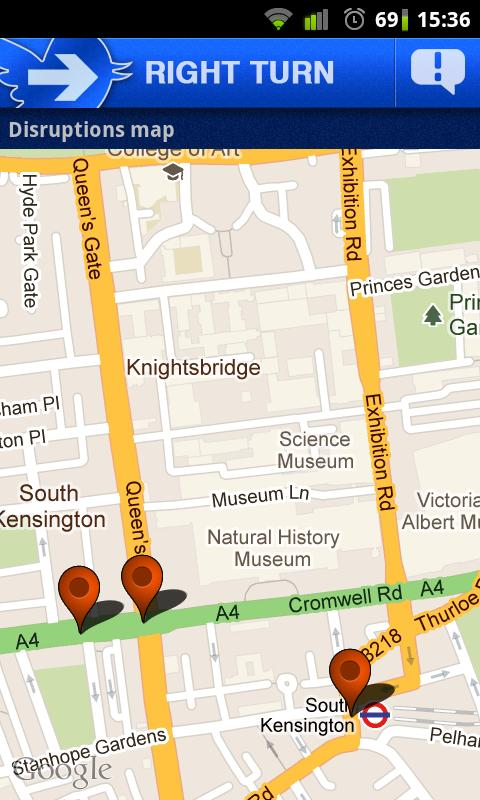
\includegraphics[width=0.4\textwidth]{images/appendix/user_interface/map_view.jpg}
\quad
\subfigure{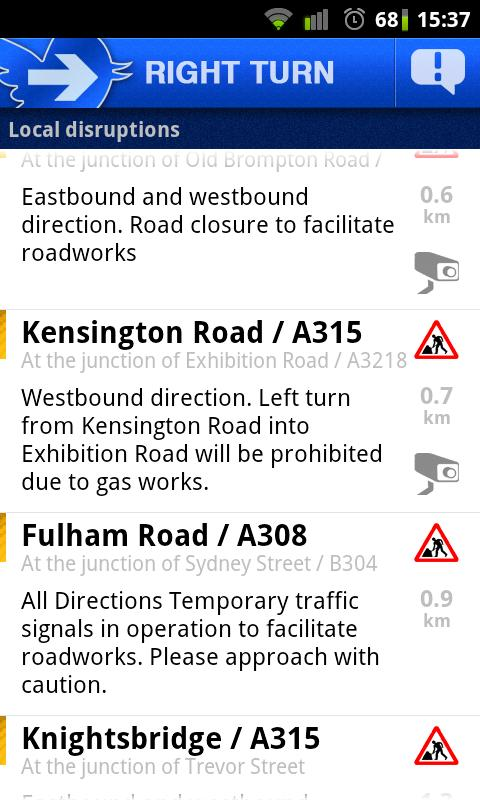
\includegraphics[width=0.4\textwidth]{images/appendix/user_interface/list_view.jpg} }}}


\mbox{\subfigure{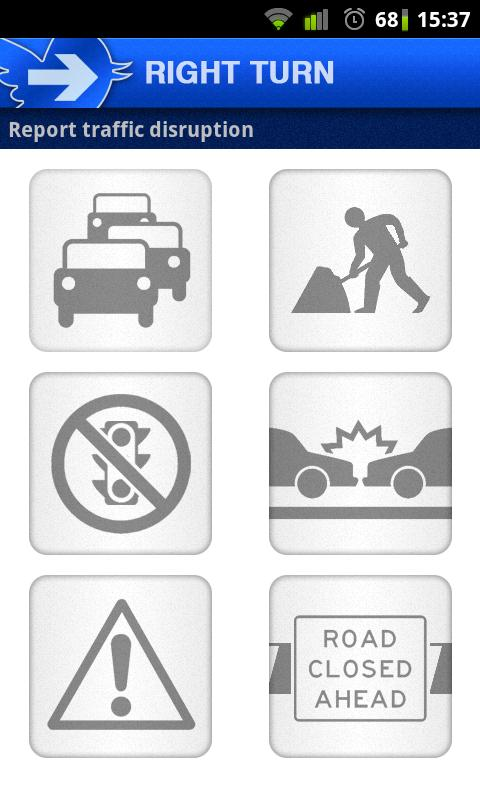
\includegraphics[width=0.4\textwidth]{images/appendix/user_interface/report_view.jpg}
\quad
\subfigure{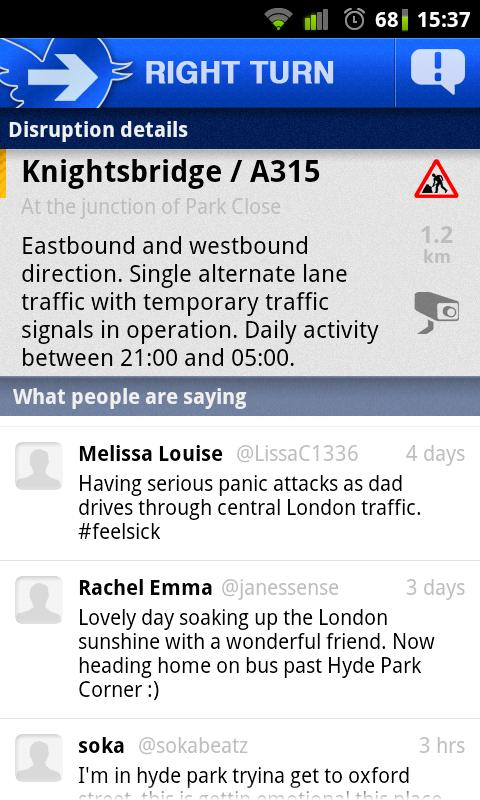
\includegraphics[width=0.4\textwidth]{images/appendix/user_interface/details_view.jpg} }}}

\caption{Examples of the implemented user interface}
\label{fig:user_interface}
\end{figure}

\begin{figure}
\centering
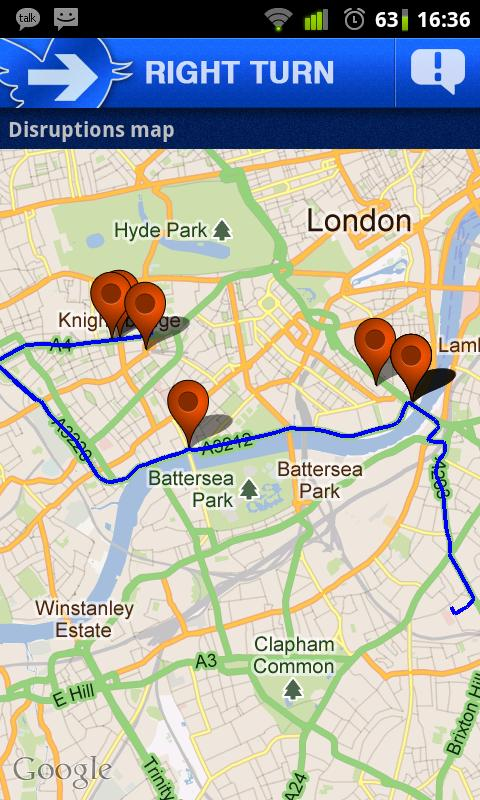
\includegraphics[width=0.45\textwidth]{images/appendix/user_interface/home_route.jpg}
\caption{Example of home route functionality}
\label{fig:home_route}
\end{figure}


\subsection{Online resources}
    \begin{description}
    \item[Github] \url{https://github.com/johnflan/Twitter-4-Traffic/} \hfill \\
        Revision control system.
    \item[Video Demonstration] \url{http://www.youtube.com/watch?v=LmWDxq2jhNI/} \hfill \\
        Video demonstration of the final product.
\end{description}

%\section{References}
%	\def\refname{}
%	\bibliography{references}
%	\bibliographystyle{plain}

\end{document}
